\newthought{\textbf{Rizki Ilhami - 2020903430042 - TRKJ 3B}}

\newday{\textbf{1 - 2 Desember 2022} - Instalasi dan Konfigurasi Hadoop}

\begin{enumerate}

\item Kendala dan Solusi
\begin{enumerate}
    \item kendala
\begin{itemize}
    \item Kendalanya pada saat menjalakan hadoop service, firefox tidak bisa dibuka.
\end{itemize}
    \item solusi
\begin{itemize}
    \item menginstal ulang firefox.
\end{itemize}
\end{enumerate}

\item Kesimpulan
\newline
    Pada Instalasi Apache Hadoop membutuhkan ruang yang
    cukup besar untuk mengekstrak file Apache Hadoop dan ram
    minimal 2gb agar bekerja optimal.


\end{enumerate}

\begin{figure}[!ht]
    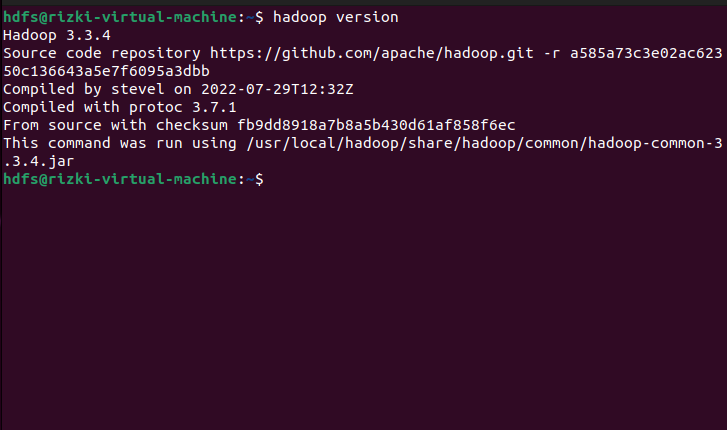
\includegraphics[width=\textwidth]{RizkiIlhami/Hadoop Version}
    \caption{hasil Hadoop}
    \label{gam:Hasil}
\end{figure}

\begin{figure}[!ht]
    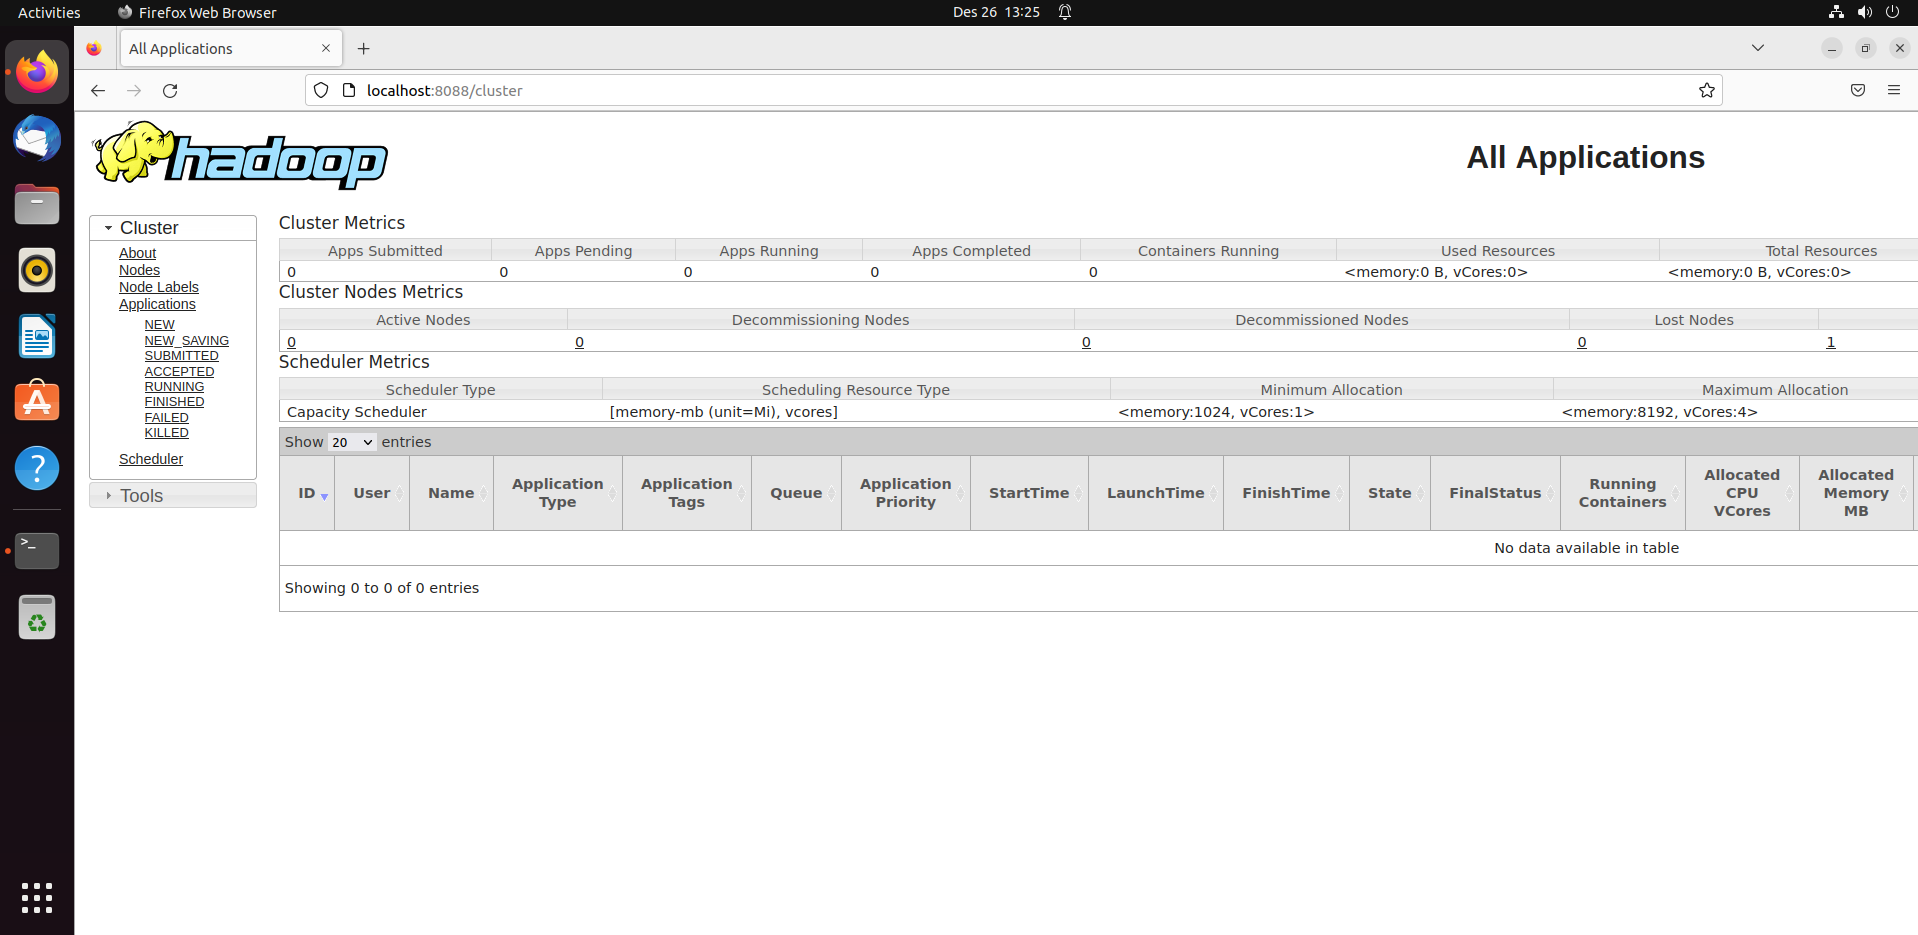
\includegraphics[width=\textwidth]{RizkiIlhami/Hadoop Web}
    \caption{hasil menjalankan Hadoop Service}
    \label{gam:Hasil}
\end{figure}

\clearpage
\newday{\textbf{8 Desember 2022} - WordCount bawaan Hadoop}
\begin{enumerate}
\item Kendala dan Solusi

\begin{itemize}
\item Tidak menemukan kendala apapun.
\end{itemize}

\item Kesimpulan
\newline
    Pada Hadoop terdapat program untuk menghitung jumlah kata 
    (WordCount) yang ada pada data. Sebagai praktikan melakukan input data terlebih
    dahulu, kemudian memprosesnya, sehingga menghasilkan data output.

\end{enumerate}

\begin{figure}[!ht]
    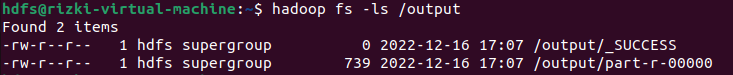
\includegraphics[width=\textwidth]{RizkiIlhami/WordCount Hadoop -ls}
    \caption{hasil WordCount bawaan hadoop}
    \label{gam:Hasil}
\end{figure}

\begin{figure}[!ht]
    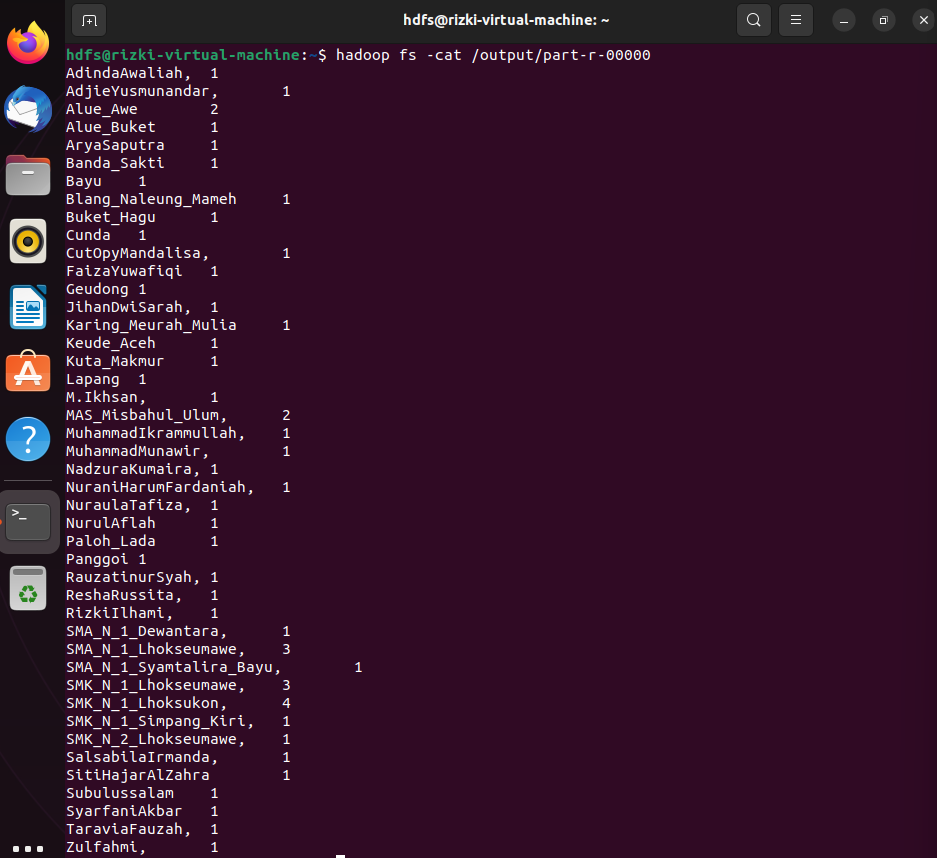
\includegraphics[width=\textwidth]{RizkiIlhami/WordCount Hadoop -cat}
    \caption{hasil WordCount bawaan hadoop}
    \label{gam:Hasil}
\end{figure}

\clearpage
\newday{\textbf{9 Desember 2022} - WordCount dengan Java}
\begin{enumerate}
\item Kendala dan Solusi

\begin{itemize}
\item Tidak menemukan kendala apapun.
\end{itemize}

\item Kesimpulan
\newline
    Untuk hasil yang ditampikan sama dengan WordCount bawaan hadoop.

\end{enumerate}

\begin{figure}[!ht]
    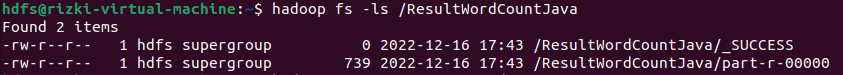
\includegraphics[width=\textwidth]{RizkiIlhami/WordCount Java -ls}
    \caption{hasil WordCount Java}
    \label{gam:Hasil}
\end{figure}

\begin{figure}[!ht]
    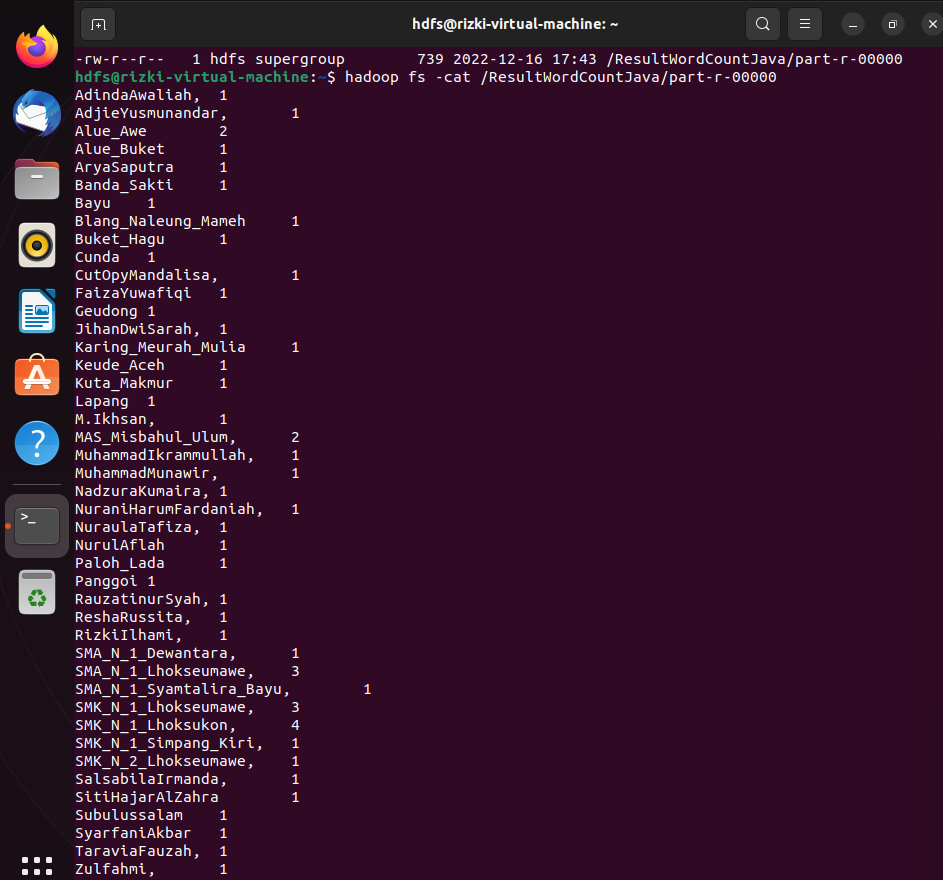
\includegraphics[width=\textwidth]{RizkiIlhami/WordCount Java -cat}
    \caption{hasil WordCount Java}
    \label{gam:Hasil}
\end{figure}


\clearpage
\newday{\textbf{15 Desember 2022} - Instalasi Apache Spark}
\begin{enumerate}
\item Kendala dan Solusi

\begin{itemize}
\item Tidak menemukan masalah apapun
\end{itemize}


\item Kesimpulan
\newline
    Apache Spark adalah sebuah framework komputasi
    yang dapat digunakan untuk mengakses data, memproses
    data, menanyakan data serta menganalisis big data

\end{enumerate}

\begin{figure}[!ht]
\includegraphics[width=\textwidth]{RizkiIlhami/spark}
\caption{hasil instalasi apache spark }
\label{gam:hasil instalasi spark}
\end{figure}

\clearpage
\newday{\textbf{16 Desember 2022} - WordCount Dengan Python}
\begin{enumerate}
\item Kendala dan Solusi

\begin{itemize}
\item Tidak bisa menjalankan {\color{red}"echo jangan heran jika orang cantik merasa jelek sementara
orang yang jelek merasa cantik | WordCountPython/map.py |
sort | WordCountPython/reduce.py"}
\end{itemize}


\item Kesimpulan
% berikan kesimpulan dari praktikum yang telah dikerjkan

\end{enumerate}

\clearpage
\newday{\textbf{22 Desember 2022} - WordCount dengan PySpark}
\begin{enumerate}
\item Kendala dan Solusi

\begin{itemize}
\item Tidak bisa menjalankan perintah {\color{red}"hadoop fs -ls /ResultWordCountPyspark"} dan {\color{red}"hadoop fs -cat /ResultWordCountPyspark/part-00000"}
\end{itemize}


\item Kesimpulan
% berikan kesimpulan dari praktikum yang telah dikerjkan

\end{enumerate}

\clearpage
\newday{\textbf{23 Desember 2022} - Machine Learning dengan PySpark}
\begin{enumerate}
\item Kendala dan Solusi

\begin{itemize}
\item
\end{itemize}


\item Kesimpulan
% berikan kesimpulan dari praktikum yang telah dikerjkan

\end{enumerate}
	